\section{Charge Transfer Properties}
We have seen that the final structure of the pentacene systems becomes more ordered and crystal-like as the quenching time is increased. It would be good now to see how this affects the charge transfer properties. A key quantity governing charge transfer rates is the ratio between electronic coupling and reorganisation energy, $\frac{H_{ab}}{\lambda}$. Seeing as we have a single molecule system, by plotting the electronic coupling we can get a qualitative view of the charge transfer dynamics and see which paths are the most likely within the structure.
%\subsection{Global Couplings}
%The global coupling distribution gives an overview of the values of coupling within the system, hence an idea of the charge transport properties of the system. To calculate these couplings I have used the analytic overlap method (AOM)\cite{gajdos_ultrafast_2014} to calculate couplings between all pairs of molecules (using a nearest neighbour cutoff) in the final snapshot of each quenched system. As can be seen from figure \ref{fig:glob_coup} more high couplings start to appear as the quench time increases. This is due to molecules packing closer in crystalline systems hence there is a larger overlap between molecular orbitals. We will see in the next section \ref{sect:couplGraphs} the microscopic structure of the coupling network for representative slices from each quenched structure. This confirms as the quench time increases larger fragments of crystalline (highly coupled) pentacene form giving rise to a better connected system. I have also plotted the global coupling distribution gathered from a simulation without electrostatics
%\begin{figure}
%	\includegraphics[width=\textwidth]{./img/DifferentQuenchTimes/GlobalCouplings.png}
%	\caption{\label{fig:glob_coup}The global coupling distribution }
%\end{figure}
\subsection{Coupling Graphs}
\label{sect:couplGraphs}
In figure \ref{fig:crystalCouplingGraph} the graph of electronic couplings between molecules has been plotted for each of the quenched systems and a crystal system after a short equilibration run with MD. In this figure the centers of mass each molecule is represented by a small black dot and the calculated coupling value with a coloured line (red, green blue). That is, if 2 molecules have a non-negligible coupling between them they would be represented by 2 black dots with either a red, green or blue line connecting them. The couplings were calculated via the analytic overlap method \cite{gajdos_ultrafast_2014} and a pertinent cluster of molecules was selected for each quench time. For the 0ns and 1ns quench times this was simply a slice 1 molecule thick in the z dimension, containing a few hundred molecules. For the 10ns and 100ns quenched structures a reasonable cluster of molecules was chosen after applying a density based clustering algorithm on the superstructure. For the crystal a plane from the crystal was chosen. All panes in figure \ref{fig:crystalCouplingGraph} show the coupling of the selected system from an angle perpendicular to the plane of molecules.
\begin{figure}
	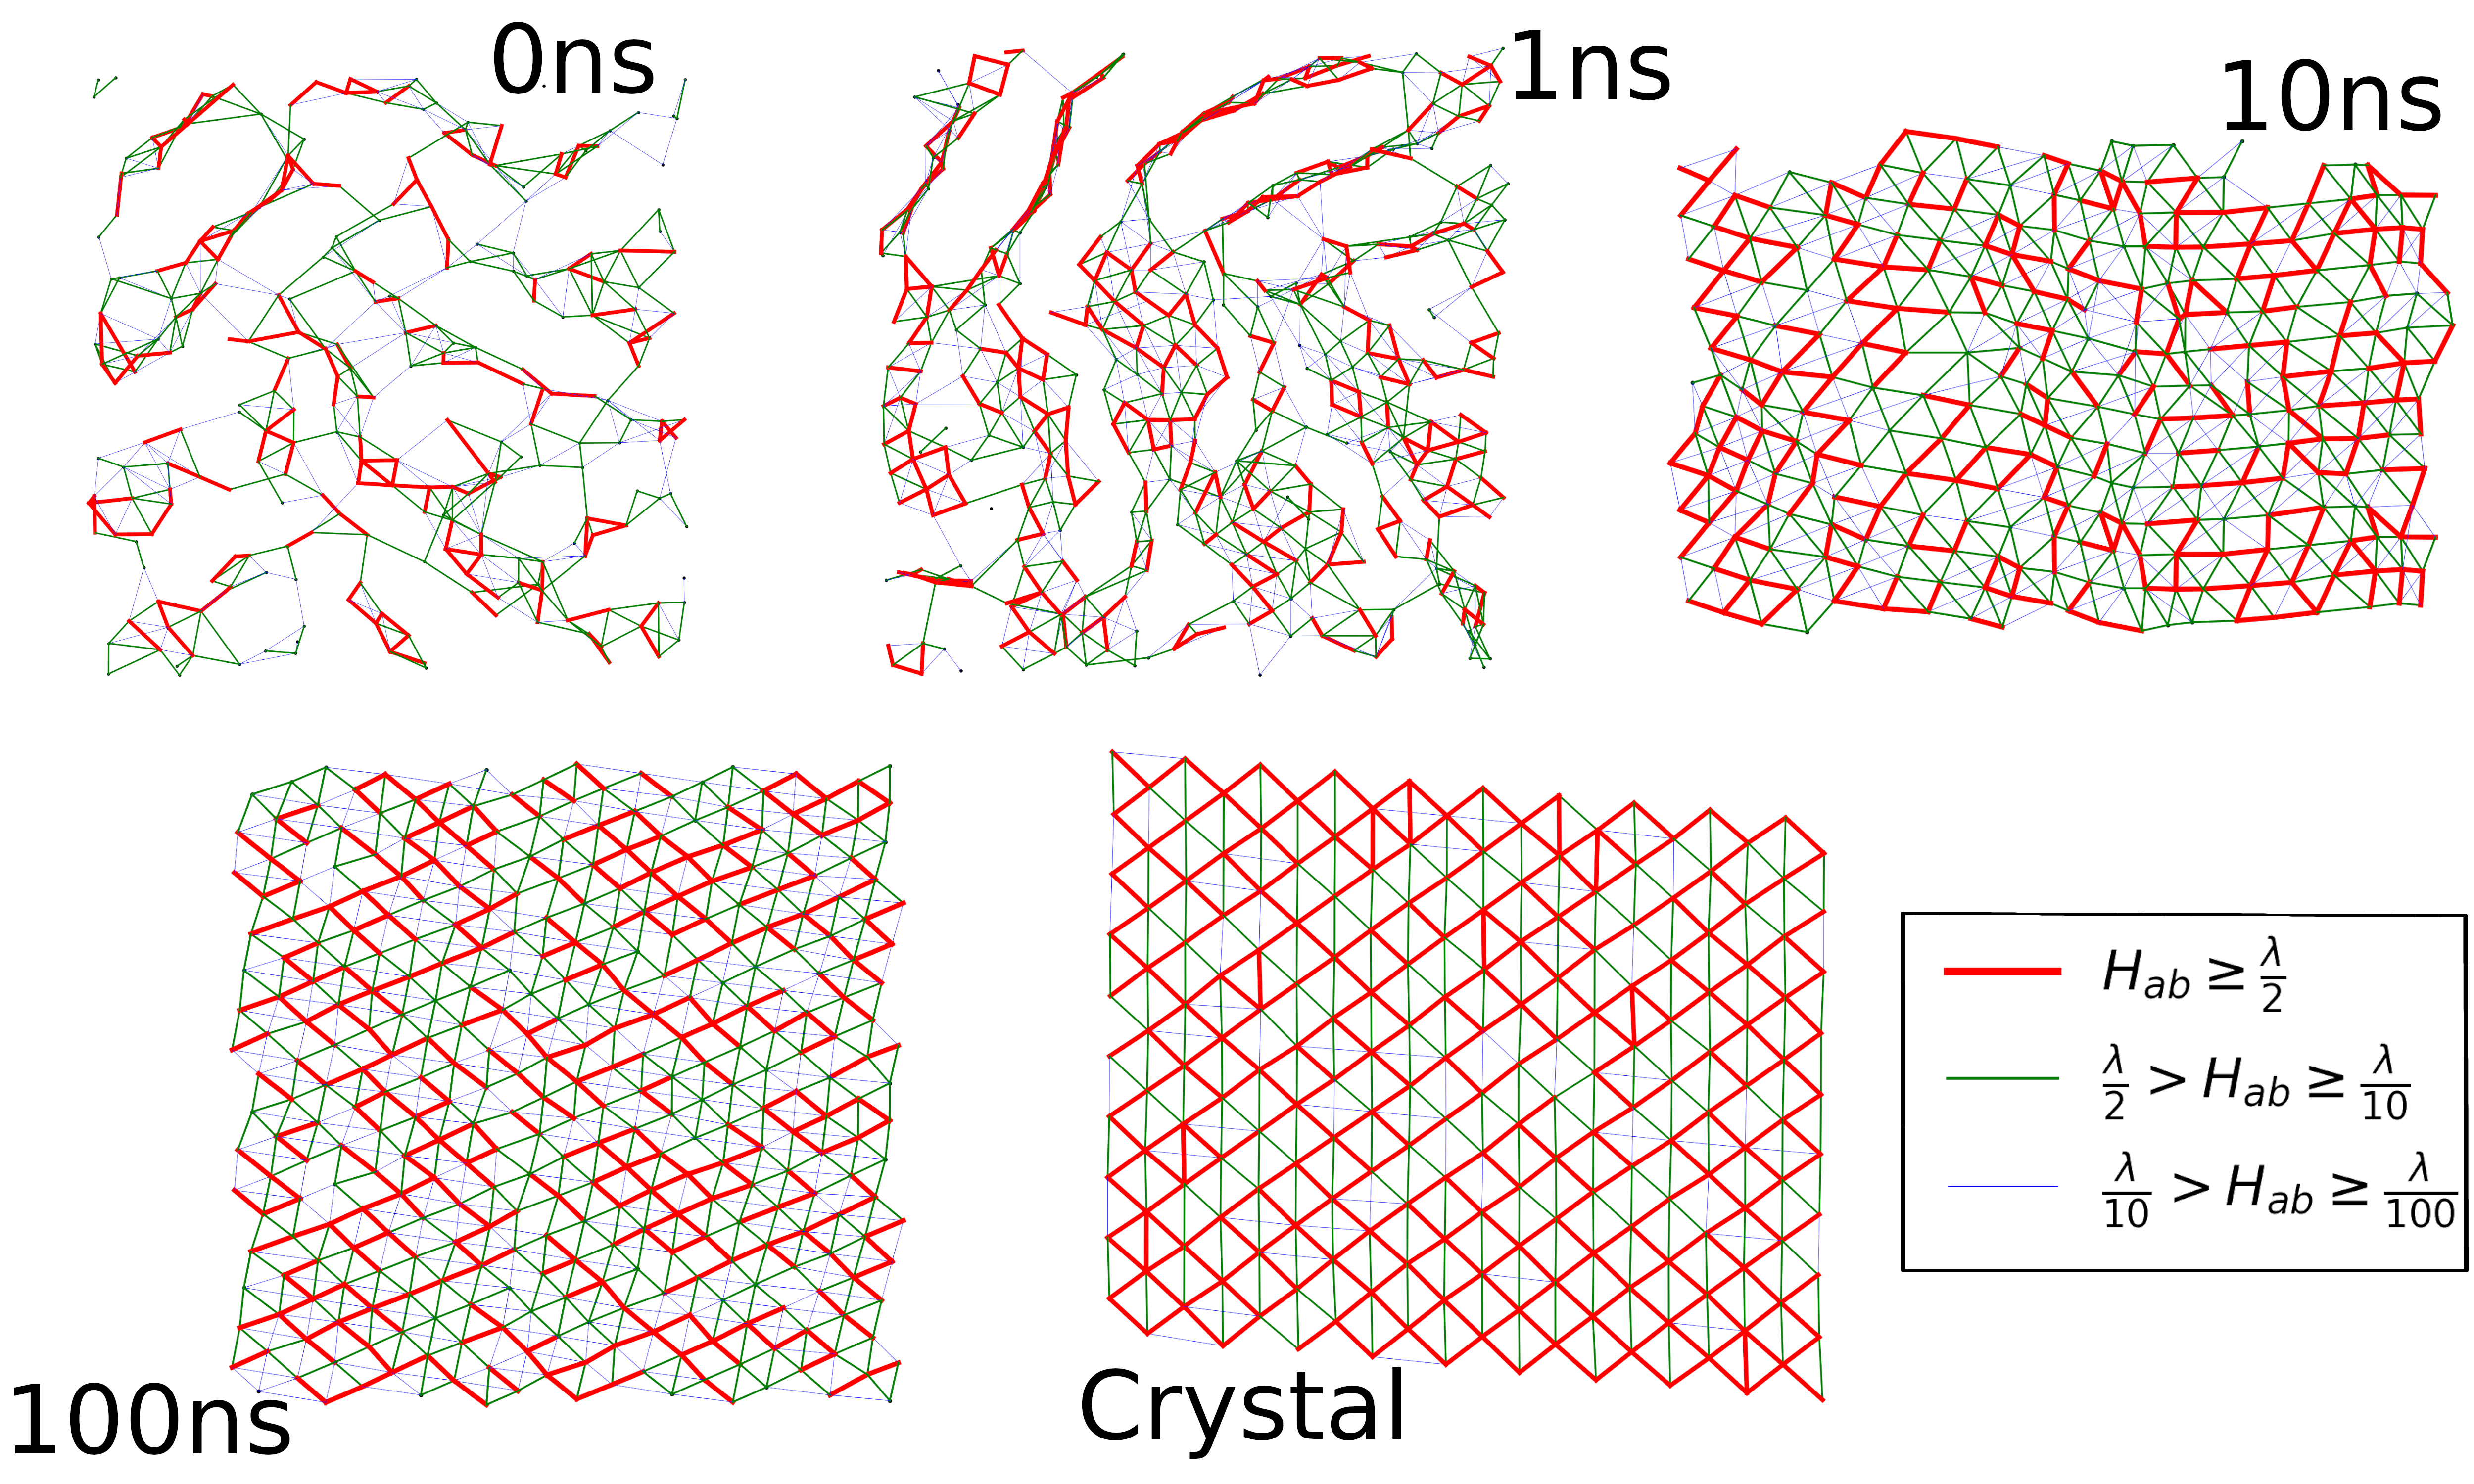
\includegraphics[width=\textwidth]{./img/CouplingPlots/CouplingGraphs_all.png}
	\caption{\label{fig:crystalCouplingGraph}A representative network of electronic coupling that each quenched structure has formed. Each structure is labelled by the quench time (e.g. 0ns, 1ns, 10ns, 100ns) or Crystal for a crystal after a short MD equilibration. Coupling strengths are categorised as high (red), medium (green) and low (blue). The definitions of the categories are given in the legend in the bottom right corner.}
\end{figure}
\\\\
We can see in the graph of the 0ns quenched structure there is very little order to the coupling network. Only very small fragments of high (red) coupling are formed and each one is connected via weak or medium coupling. We can define a 'high coupling fragment' as any set of molecules which can all be reached from any member of the set via an unbroken path of high coupling. The mean size of these high coupling fragments in the 0ns structure is 4.1 molecules and there are 503 of them. In this structure we would expect to see a localised polaron (over a $\sim$ 3 molecules) and low mobilities due to the lack of conductive channels in the structure. The mean size of fragments increases and the number of fragments decreases as we increase the quenching time as shown in table \ref{tab:cluster_sizes}.
\\
\begin{table}[h]
	\begin{tabular}{cccc}
		\textbf{Quench Time} [ns] & \textbf{Mean Fragment Size} & \textbf{Fragment Size Std Dev} & \textbf{Num Fragments} \\
		\hline &&&\\
		0 & 4.2 & 3.8 & 503 \\
		1 & 4.5 & 5.0 & 493 \\
		10 & 6.5 & 9.3 & 373 \\
		100 & 8.7 & 16.2 & 292 \\
		\hline &&&\\
	\end{tabular}
	\caption{\label{tab:cluster_sizes}The change in the number of high coupling fragments, and the mean and standard deviation of their size, found in each structure as the quenching time was varied.}
\end{table}
\\
We can see in table \ref{tab:cluster_sizes} that as the quenching time increases, the size of the highly coupled fragments (how many molecules are connected) increases and fewer of them are formed. The standard deviation also increases showing in the 0ns quenched structure most fragments are very small but as we increase the quench time we still get smaller fragments but much larger ones can now form too. These larger fragments can act as regions of high conductivity allowing much larger mobilities to be achieved than in the quicker quenching times.

\subsection{Hole Mobilities}
\label{sect:mobilities}
To properly quantify the charge transfer dynamics the electron-hole mobility can be calculated on the output of a surface hopping simulation. A full discussion of the calculation of the electron mobility can be found here in Giannini, 19 \cite{Giannini2019}. The mean squared displacement (MSD) of the charge carrier wavefunction was calculated and the gradient found by fitting a straight line to this. The gradient of the MSD, which is proportional to the Einstein diffusion coefficient D, was then used to calculate the mobility as in equation \eqref{eq:mobility} below.
\begin{equation}
	\mu_{ij} = \frac{e D_{ij}}{k_{B} T}
	\label{eq:mobility}
\end{equation}
Where $D_{ij}$ represents the Einstein diffusion coefficient, $k_{B}$ is the Boltzmann constant, $e$ the elementary charge and $T$ is the temperature.
\subsection{Simulation Set up}
\begin{wrapfigure}{r}{0.38\textwidth}
	\vspace*{-0.7cm}
	\centering
	\includegraphics[width=0.2\textwidth]{./img/RestraintsPos.png}
	\caption{\label{fig:rest}The restraint set up for 1 molecule. Each coloured zig-zag shows the atoms that are restrained.}
\end{wrapfigure}
\vspace*{0.5cm}
The surface hopping simulations require a swarm of hundreds of independent trajectories ($\sim$200), each with slightly different positions and velocities to fully sample phase space. The code currently does not support electrostatic interactions, so, in order to maintain the structure from the molecular dynamics simulations, center of mass restraints were used on each molecule. The restraint set up for 1 molecule is shown in figure \ref{fig:rest}. Here each of the 4 coloured zig-zag shapes show which atoms are restrained. These atoms were restrained about their center of mass. This configuration of restraints was used in order to stop rotations about the long axis for each molecule as this would allow molecules to form a face-to-face stacking giving rise to unphysically high couplings.
\\\\
The restraints were tested ... Sam tested similar restraints
\\\\
In order to obtain initial positions and velocities for the individual trajectories an MD equilibration was carried out using the restraint set up. This was carried out for 220ps using the NVE ensemble. The first 4ps were discarded and positions and velocities were then sampled every 1ps in order to get 216 trajectories. When these 216 trajectories were created, the Hamiltonian was calculated for each. This allowed and adiabatic state to be selected which, when transformed to the diabatic basis gave a population close to the center of the system and had an energy within 3KT of the ground state energy. An explanation of how this was done is given in appendix \ref{ap:AdiabaticSelector}. In short the method consisted of finding the adiabatic energy (eigenvalue) and diabatic populations (eigenvector) corresponding to adiabatic state n which yielded a state both close to the center and within approximately 3KT of the ground state energy. This was done to ensure a quick convergence of the mean squared displacement of the charge carrier. The surface hopping simulations were then carried out with initial positions and velocities coming from the NVE equilibration run and the initial wavefunction being selected as mentioned above. Other parameters were taken from previous surface hopping simulations carried out by other members of the group.

\subsubsection{0ns and 1ns Systems}
The region selected to run the surface hopping calculations on was important in order to get a fair representation of the mobilities achievable within each structure. In the 0ns and 1ns quenched structures 6 slices were selected from the final snapshot of the structure

\clearpage
\subsection{Molecular Dynamics without Partial Charges}


\label{sect:partial_charge_importance}

